\documentclass[12pt]{article}

\usepackage{sbc-template}

\usepackage{graphicx,url}

\usepackage[brazil]{babel}   
%\usepackage[latin1]{inputenc}  
\usepackage[utf8]{inputenc}  
% UTF-8 encoding is recommended by ShareLaTex
\usepackage{verbatim}
\usepackage{listings}
\usepackage{xcolor}

\usepackage{graphics} % for pdf, bitmapped graphics files
\usepackage{mathptmx} % assumes new font selection scheme installed
\usepackage{times} % assumes new font selection scheme installed
\usepackage{amsmath} % assumes amsmath package installed
\usepackage{amssymb}  % assumes amsmath package installed
\definecolor{verde}{rgb}{0,0.5,0}

%para customizar o código (ver https://en.wikibooks.org/wiki/LaTeX/Source_Code_Listings)
\lstset{language=C, %defina a linguagem usada no trabalho
              belowcaptionskip=1\baselineskip,
                breaklines=true,
                frame=false,
                xleftmargin=\parindent,
                showstringspaces=false,
                basicstyle=\footnotesize\ttfamily,
                keywordstyle=\bfseries\color{green!40!black},
                commentstyle=\itshape\color{purple!40!black},
                identifierstyle=\color{blue},
                stringstyle=\color{orange},
                numbers=left,
            }

\sloppy

\title{Improving end joint force sensing for robotic grasping\\
(Using IMUs to estimate contact force)}

\author{Nao Ouyang}
\address{Rotation in Harvard Biorobotics Lab}




%\nextinstitute
%  Department of Computer Science -- University of Durham\\
%  Durham, U.K.
%\nextinstitute
 % Departamento de Sistemas e Computação\\
  %Universidade Regional de Blumenal (FURB) -- Blumenau, SC -- Brazil

\begin{document} 

\maketitle

\begin{introduction}
    This is my final report for my 299r rotation during Spring 2018 in Prof. Robert Howe's lab.
\end{introduction}
%\begin{abstract} 
    
%\end{abstract}

\section{Introduction}

State-of-the art robots are bad at grasping in unstructured environmnents, limiting their use to
structured environments like factory floors. An active area of research in order for robots to expand to unstructured
environments (such as kitchens or hospital environments),  is the ability to grasp
novel objects (objects the robot has not encountered before and may not have any prior information
about). Grasp stability analysis plays a critical role in enabling robots to achieve high grasping
success rates (in terms of not dropping objects). Through sensing, for instance tactile sensing, we
can predict whether or not we will drop the object after grasping and prior to moving. If we find
our grasp to be unstable, and assuming the object has not moved during grasping such that releasing
our grip might e.g. cause it to tumble, we can simply release our grasp and try again. 

Physical model approaches involve modeling the contact forces, contact location, and surface normals
(which will differ from the force XYZ if the surface(s) are squishy). However, over the last few
decades physical models have proven insufficient, in part due to complex gripper-object interactions
during grasping which are both difficult to measure and hard to model. Thus, one of the aspects of
this investiation.

During the course of this rotation, senior gad student Qian Wan discoverd 

\section{Referencial Teórico} \label{sec:firstpage}

A primeira página deve apresentar o título do trabalho, o nome e o endereço (institucional) dos autores, o resumo em portutguês e o “abstract” em inglês. O título deve ser centralizado, em fonte no estilo negrito e tamanho 16pts, com 12pts de espaçamento antes do início da linha do título. 

Os nomes dos autores devem ser centralizados, todos dispostos na mesma linha, em fonte 12pt, negrito, separados por vírgulas e com 12pts de espaço entre o título. 

O endereço institucional dos autores deve ser centralizado, em fonte 12pt, também com 12pts de espaço depois dos nomes dos autores. Os endereços de e-mail devem ser escritos usando fonte estilo “Courier New”, tamanho 10 pontos, com 6 pontos de espaço antes e 6 pontos de espaço depois da linha dos endereços de e-mail.

O abstract e o “resumo” (se for o caso) devem ser escritos em fonte Times, tamanho 12, tabulado em 0.8cm em ambos os lados. As palavras \textbf{Abstract} e \textbf{Resumo} devem ser escritas em negrito e devem preceder o texto.

\subsection{Sobre o Referencial teórico}
O Referencial teórico é a fundamentação do estudo/pesquisa. Os assuntos teóricos explorados pelos alunos nesta seção devem ter relação direta com o tema da pesquisa e estar alinhados aos objetivos traçados.

Nesta seção, o aluno pode abordar também os estudos relacionados ao tema. É importante o uso de artigos publicados em anais e periódicos recentes.


\section{Metodologia}

Descreve os métodos e técnicas utilizados na pesquisa

\subsection{Sobre seções e parágrafos}

Os títulos das seções devem estar em negrito, fonte 13pt, alinhados a esquerda. A linha do título da seção deve possuir 12pts de espaçamento antes do seu início. A numeração das seções é opcional, embora recomendado. O primeiro parágrafo de cada seção não deve ser tabulado, enquanto que as primeiras linhas dos parágrafos subsequentes devem ser tabulados em 1.27 cm.

Os títulos das subseções devem estar em negrito, 12pt, alinhados a esquerda.


\section{Análise dos dados}\label{sec:analisedosdados}

Nesta seção, o aluno descreve o efetivo procedimento metodológico adotado e aponta os resultados da pesquisa. Na análise de dados, é  aconselhável o uso de tabelas, figuras, linhas de códigos etc para representar os resultados do estudo.

As Tabelas, Quadros e Figuras, assim como as legendas de Tabelas, Quadros e Figuras devem estar centralizadas se conterem apenas em uma linha (Figura~\ref{fig:figura1}), caso contrário devem estar tabuladas em 0.8cm em ambas as margens, como mostra a Figura~\ref{fig:figura2}. 

\begin{figure}[ht]
\centering
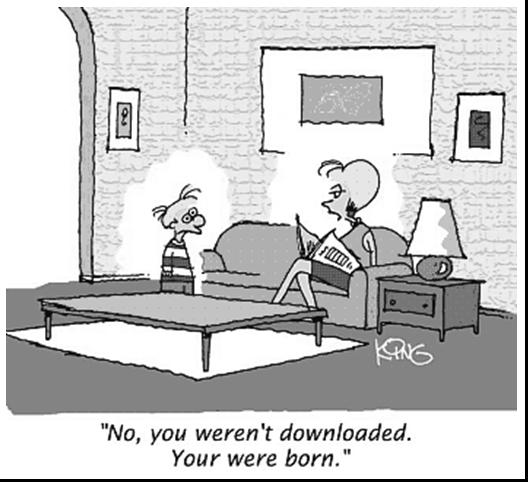
\includegraphics[width=.3\textwidth]{fig1.jpg}
\caption{Exemplo de figura}
\label{fig:figura1}
\end{figure}

As legendas devem ser escritas na fonte “Helvetica”, Tamanho 10pts, negrito, com espaço de 6pts antes e depois de cada legenda. Sempre que possível, procure colocar a figura delimitada por um quadro (Figura~\ref{fig:figura1} e Figura~\ref{fig:figura2})

\begin{figure}[!ht]
\centering
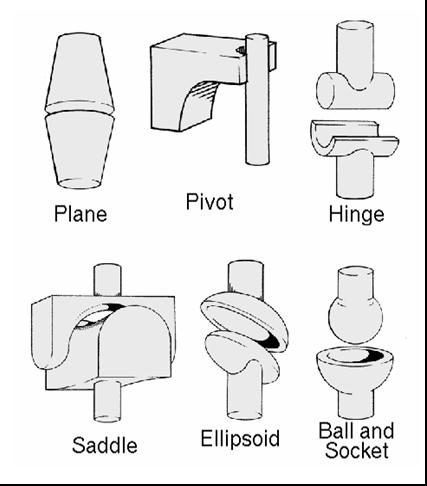
\includegraphics[width=.2\textwidth]{fig2.jpg}
\caption{Essa figura foi referenciada na Seção~\ref{sec:analisedosdados}.}
\caption{Fonte: SBC.}
\label{fig:figura2}
\end{figure}

Em tabelas, tente evitar o uso de fundos coloridos ou preenchidos, assim como linhas duplas na borda, ou linhas desnecessárias. Quando \cite{knuth:84} relatar dados empíricos, não faça uso de mais dígitos decimais do que o necessário. A legenda da tabela deve ser colocada antes da tabela (veja Tabela 1) e a fonte usada na legenda deve ser Helvetica, tamanho 10pts, negrito, com 6pts de espaço antes e depois de cada legenda.

\begin{table}[!ht]
\centering
\caption{Exemplo de tabela de 3 colunas e 2 linhas}
\label{tab:exTable1}
\smallskip
\begin{tabular}{l c c}
\hline
& Value 1 & Value 2\\[0.5ex]
\hline
&&\\[-2ex]
Case 1 & 1.0 $\pm$ 0.1 & 1.75$\times$10$^{-5}$ $\pm$ 5$\times$10$^{-7}$\\[0.5ex]
\hline
&&\\[-2ex]
Case 2 & 0.003(1) & 100.0\\[0.5ex]
\hline
\end{tabular}
\end{table}

\subsection{Código fonte}
A inserção de código fonte deve ser por meio

\begin{lstlisting}

int main(){
  int a,b,c;
  float x;
  printf("informe o tamanho do lado do quadrado");
  scanf("%d", &a);
  printf("A area do quadrado %d", b=area(a));
  printf("Duas vezes o valor do lado do quadrado %d", c=aumenta(a));

\end{lstlisting}



\section{Considerações Finais}

Referências bibliográficas devem ser utilizadas dentro de um estilo uniforme e não ambíguo. A SBC sugere os seguintes formatos para referências: \cite{knuth:84}, \cite{boulic:91}, e \cite{smith:99}.

\bibliographystyle{sbc}
\bibliography{sbc-template}

\end{document}
